\documentclass{beamer}
\usepackage[czech]{babel}
\usepackage{hyperref}
\usepackage{graphicx}
\usepackage{textpos}
\title{Spam Filter}
\subtitle{Semestrální úloha z RPH}
\author[Jakub Ambroz a Kateřina Kučerová]{Jakub Ambroz a Kateřina Kučerová\\ 
\includegraphics[height=2cm]{logo.png}}
\institute[ČVUT]{České vysoké učení technické}
\date{\today}

\usetheme{Malmoe}
\usecolortheme{whale}
\setbeamertemplate{enumerate items}[default]
\setbeamertemplate{itemize items}[default]

\addtobeamertemplate{frametitle}{}{%
\begin{textblock*}{100mm}(.98\textwidth,-0.7cm)

\includegraphics[height=0.6cm]{logo.png}
\end{textblock*}}

\begin{document}
	\begin{frame}
		\maketitle
	\end{frame}
\section{Spam filter}	
\begin{frame}
\frametitle{Úvod}
\begin{itemize}
\item Knihovna emails k rozdělení textu souboru na části
\item Tokenizace pomocí "str.replace" a \emph{regular expression} k odstranění html tagů
\item Rozdělení na slova
\end{itemize}
\end{frame}
\begin{frame}
	\frametitle{Popis}
	\begin{itemize}
		\item Náš filtr funguje na principu počítání četnosti výskytu slov ve spamech a v hamech. Pak počítá jestli je slovo v testovaném emailu častěji v spamech či v hamech
		\item Využití metadat o emailu stejným způsobem
		\item Spojení obou pravidel logickým and - odstranění většiny False Positives
	\end{itemize}
\end{frame}
\begin{frame}
	\frametitle{Testovací sada}
	\begin{itemize}
		\item Vytvoření náhodné trénovací a testovací. Napůl pomocí pythonu napůl příkazové řádky
	\end{itemize}
	\begin{figure}
		\centering
		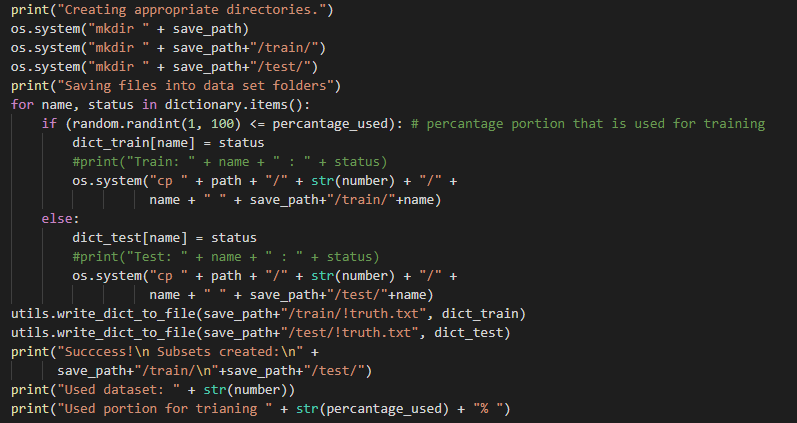
\includegraphics[width=1\textwidth]{shell.png}
	\end{figure}
\end{frame}

\section{Spolupráce}
\begin{frame}
\frametitle{Spolupráce: GitLab}
\begin{figure}
	\centering
	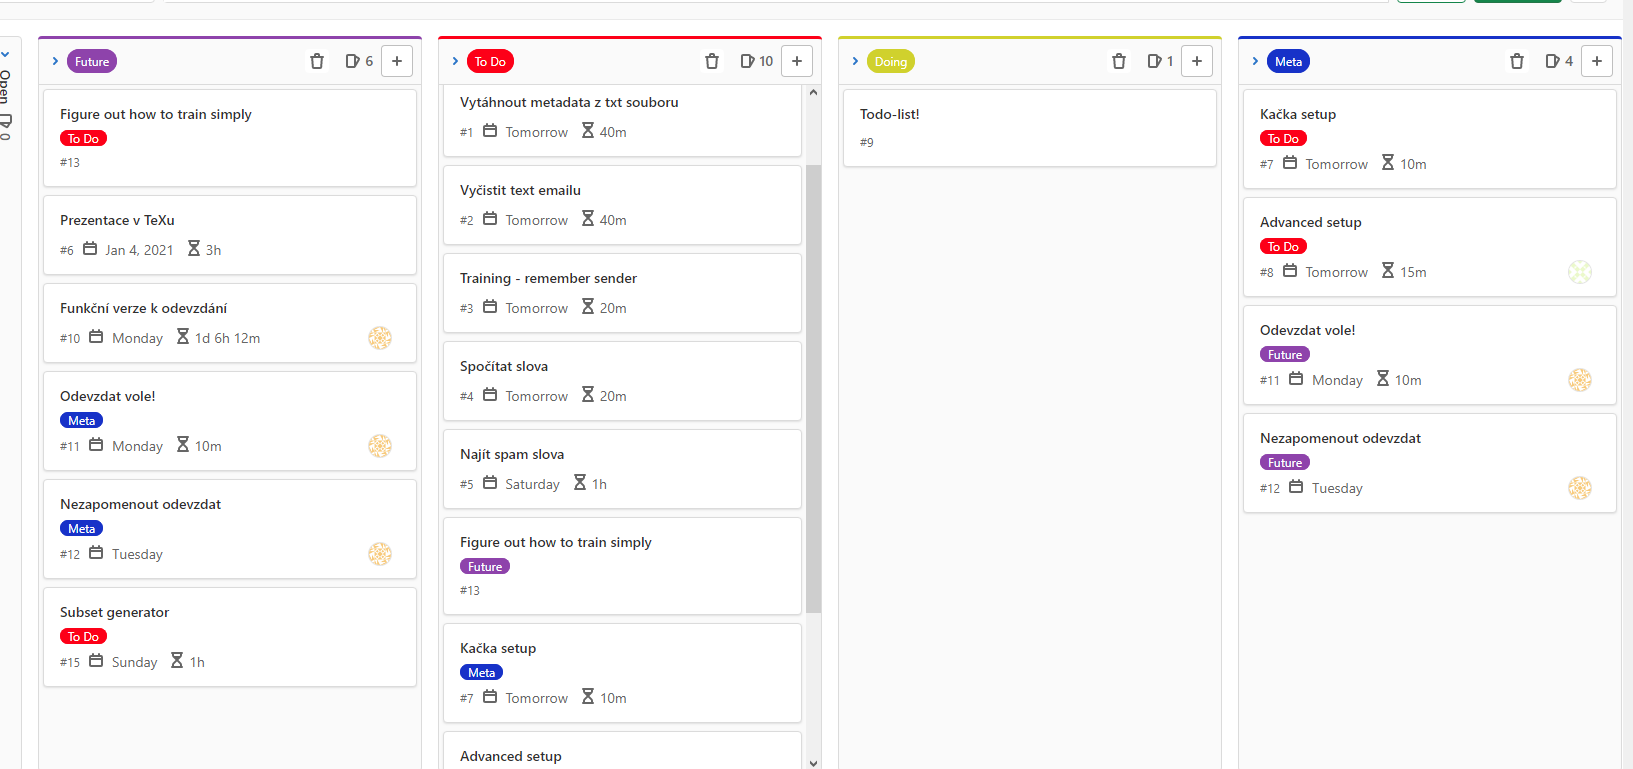
\includegraphics[width=1\textwidth]{TODO_LIST.png}
\end{figure}
\end{frame}

\begin{frame}
    \frametitle{Spolupráce: VSCode - Liveshare}
\begin{figure}
	\centering
	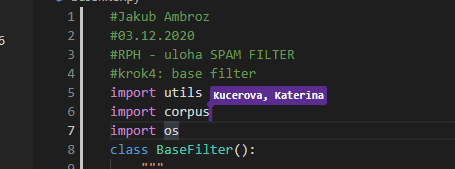
\includegraphics[width=1\textwidth]{liveshare2.png}
\end{figure}
\end{frame}
\begin{frame}
	\frametitle{Výsledky}
	\begin{figure}
		\centering
		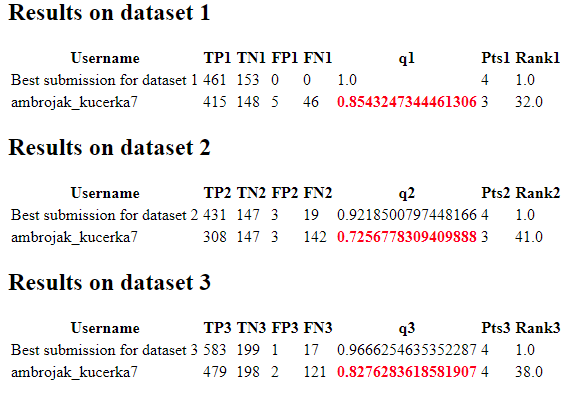
\includegraphics[width=1\textwidth]{results.png}
	\end{figure}
\end{frame}
\end{document}